\documentclass{article}
\usepackage[utf8]{inputenc}
\usepackage{hyperref}
\usepackage[letterpaper, portrait, margin=1in]{geometry}
\usepackage{enumitem}
\usepackage{amsmath}
\usepackage{booktabs}
\usepackage{graphicx}
\usepackage{mathtools}  
\usepackage{diffcoeff} 
\usepackage{hyperref}
\usepackage{physics}
\hypersetup{
colorlinks=true,
    linkcolor=black,
    filecolor=black,      
    urlcolor=blue,
    citecolor=black,
}
\usepackage{natbib}

\usepackage{titlesec}
\usepackage{chngcntr}

\counterwithin*{equation}{section}
\counterwithin*{equation}{subsection}


  
\title{Homework 3 }
\author{Economics 7103}
\date{Spring semester 2023}
  
\begin{document}
  
\maketitle

\section{}
The proof can be shown by simple log rules manipulation:\newline

Given:

\begin{equation}
y_i = e^\alpha\delta^{d_i}z^\gamma_ie^{\eta_i}
\end{equation}

Taking natural log on both side:
\begin{equation}
    \ln(y_i) = \ln(e^\alpha\delta^{d_i}z^\gamma_ie^{\eta_i})
\end{equation}

Expanding further:

\begin{equation}
\ln(y_i) = \alpha\ln(e) + \ln(\delta)d_i + \gamma\ln(z_i) + \eta_i\ln(e)      
\end{equation}
\newline

We know that the natural log of Euler's number is 1 
\newline

Thus:

\begin{equation}
    \ln(yi) = \alpha + \ln(\delta)d_i + \gamma\ln(z_i) + \eta_i
\end{equation}

Hence Proved.
\newline
\newline

\section{}
 \(\delta\) is the coefficient to the binary variable that indicates the treatment/control 
group. In the control group, when $d_i = 0$ then \(\delta\) does not exist. But when it is 1, \(\delta\) gives us the multiplier effect for energy consumption of being in the treated group.   
\newline
\newline

\section{}
The change in $y_i$ with respect to change in $d_i$ tells us the amount of electricity saved due to being in the treatment group.
\newline

\begin{equation}
    \frac{\Delta y_i}{\Delta d_i} =  y_1 - y_0
\end{equation}

\begin{equation}
   \hspace{3cm} = e^\alpha\delta^{d_i}z^\gamma_ie^{\eta_i} - e^{\alpha}z^\gamma_ie^{\eta_i}
\end{equation}

\begin{equation}
   \hspace{20mm} = (\delta - 1)e^{\alpha}z^\gamma_ie^{\eta_i}
\end{equation}

Multiplying both sides with $y_i$:

\begin{equation}
   \hspace{40mm} = (\delta - 1)e^{\alpha}z^\gamma_ie^{\eta_i}* \frac{e^\alpha\delta^{d_i}z^\gamma_ie^{\eta_i}}{e^\alpha\delta^{d_i}z^\gamma_ie^{\eta_i}} 
\end{equation}

This gives us: 

\begin{equation}
   \hspace{10mm} = \frac{\delta - 1}{\delta^{d_i}}y_i
\end{equation}

Hence Proved.
\newline
\newline

\section{}
The partial derivative tells us the effect of one unit change in $z_i$, the size of home in square feet, on electricity consumption $y_i$. 

\begin{equation}
    \pdv{y_i}{z_i} = e^\alpha\delta^{d_i}e^{\eta_i}(\pdv{z^\gamma_i}{z_i})
\end{equation}

\begin{equation}
   \hspace{15mm} = e^\alpha\delta^{d_i}e^{\eta_i} * \gamma  * z^{\gamma_i - 1}
\end{equation}

Multiplying both sides by $z_i$:

\begin{equation}
   \hspace{8mm} = \frac{\gamma}{z_i} * e^\alpha\delta^{d_i}z^\gamma_ie^{\eta_i}
\end{equation}

This is the same as $y_i$

\begin{equation}
   \hspace{-10mm} = \gamma \frac{y_i}{z_i}
\end{equation}

Hence proved.
\newline
\newline
\newline
\newline
\newline
\newline
\newline
\newline
\newline
\newline
\newline
\newline
\newline
\newline
\newline


\section{}

The table gives us the Coefficients for log regressions as well as the marginal effects (dy/dx).
\newline

\begin{table}[ht]
    \centering
    {
\def\sym#1{\ifmmode^{#1}\else\(^{#1}\)\fi}
\begin{tabular}{l*{1}{c}}
\hline\hline
                    &\multicolumn{1}{c}{(1)}\\
                    &\multicolumn{1}{c}{}\\
                    &Mean/Std. Dev.\\
\hline
Variable 1          &       11.69\\
                    &     (10.36)\\
Variable 2          &       20.67\\
                    &     (14.46)\\
Outcome variable    &      208.29\\
                    &    (158.39)\\
\hline
Observations        &         100\\
\hline\hline
\end{tabular}
}

    \caption{Regression estimates (ls: ln(sqrt), lt: ln(temp))}
    \label{tab:my_label}
\end{table}

\section{}
See below.
\begin{figure}[ht]
    \centering
    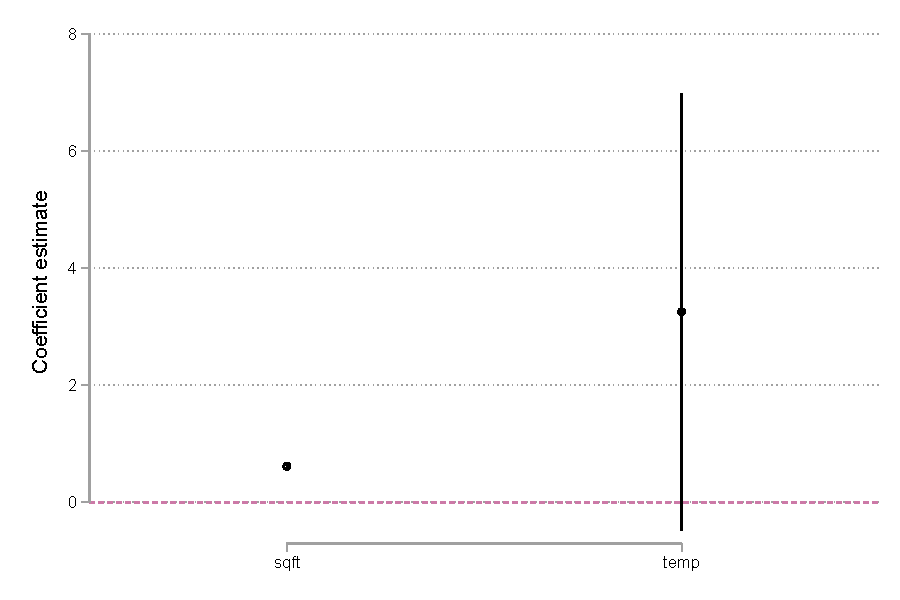
\includegraphics{graph.pdf}
    \caption{Marginal effects with bootstrapped CI}
    \label{fig:my_label}
\end{figure}






\end{document}